% !TEX root = diplomarbeit.tex
\chapter{Kommunikation Applikation und Hexacopter}
\renewcommand{\kapitelautor}{Autor: Katharina Joksch, Lucas Ullrich}
Um zwischen dem Hexacopter und dem Server eine Verbindung herzustellen wird eine Kommunikationsschnittstelle benötigt. Diese muss Drahtlos arbeiten und einen größeren Bereich
abdecken. Über diese werden anschließend die diversen Daten übertragen, dazu zählen \zB die Route, \bzw der Name des Gastes.

%%%%%%%%%%%%%%%%%%%%%%%%%%%%%%%%%%%%%%%%%%%%%%%%%%%%%%%%%%%%%%%%%%%%%%%%%%%%%%%
\section{Allgemeine technische Planung}
In der Planung wurde eine unkomplizierte und verlässliche Lösung für beide Kommunikationspartner gesucht. Da Bluetooth kaum noch standardmäßig verbaut wird hier wiederum
Serverseitig eine externe Hardware benötigt, um dies zu vermeiden wurde WLAN ins Auge gefasst.

WLAN stellte sich folglich als ideale Schnittstelle heraus,
es gibt die Möglichkeit zu Handover in sehr großen Bereichen, es ist nach einmaligem Setup vergleichsweise unkompliziert und es bietet diverse Möglichkeiten um festzustellen
ob die Verbindung noch aufrecht ist.

%%%%%%%%%%%%%%%%%%%%%%%%%%%%%%%%%%%%%%%%%%%%%%%%%%%%%%%%%%%%%%%%%%%%%%%%%%%%%%%
\section{Schnittstelle Hexacopter}
Seitens des Hexacopters wird ein zusätzliches Modul benötigt, dieses muss über eine der Schnittstellen des Mikrocontrollers ansprechbar sein.

  \subsection{Technische Planung}
  Bei der Planung wurde darauf geachtet ein WLAN-Modul zu wählen welches bekannter maßen funktioniert \bzw ein entsprechender Support zur Verfügung steht.
  So fiel die Wahl auf das WLAN-Modul RN171, vertrieben durch Microchip, hergestellt von Roving Networks.

  Das gewählte WLAN-Modul wird über eine UART-Schnittstelle angesteuert und verfügt über einige frei konfigurierbare Pins, diese werden schließlich zum Überwachen der
  Verbindung verwendet.

  \subsection{Umsetzung}
  Bei der Umsetzung stand für die anfänglichen Tests ein Evaluation-Kit zur Verfügung. Dieses kann ohne weitere Hardware direkt über ein USB-Kabel mit einem PC verbunden werden.
  So ist es möglich die nötigen Konfigurationen des Moduls auszutesten bevor dieses in der Hardware implementiert wird.

  \begin{figure}[H]
    \begin{centering}
      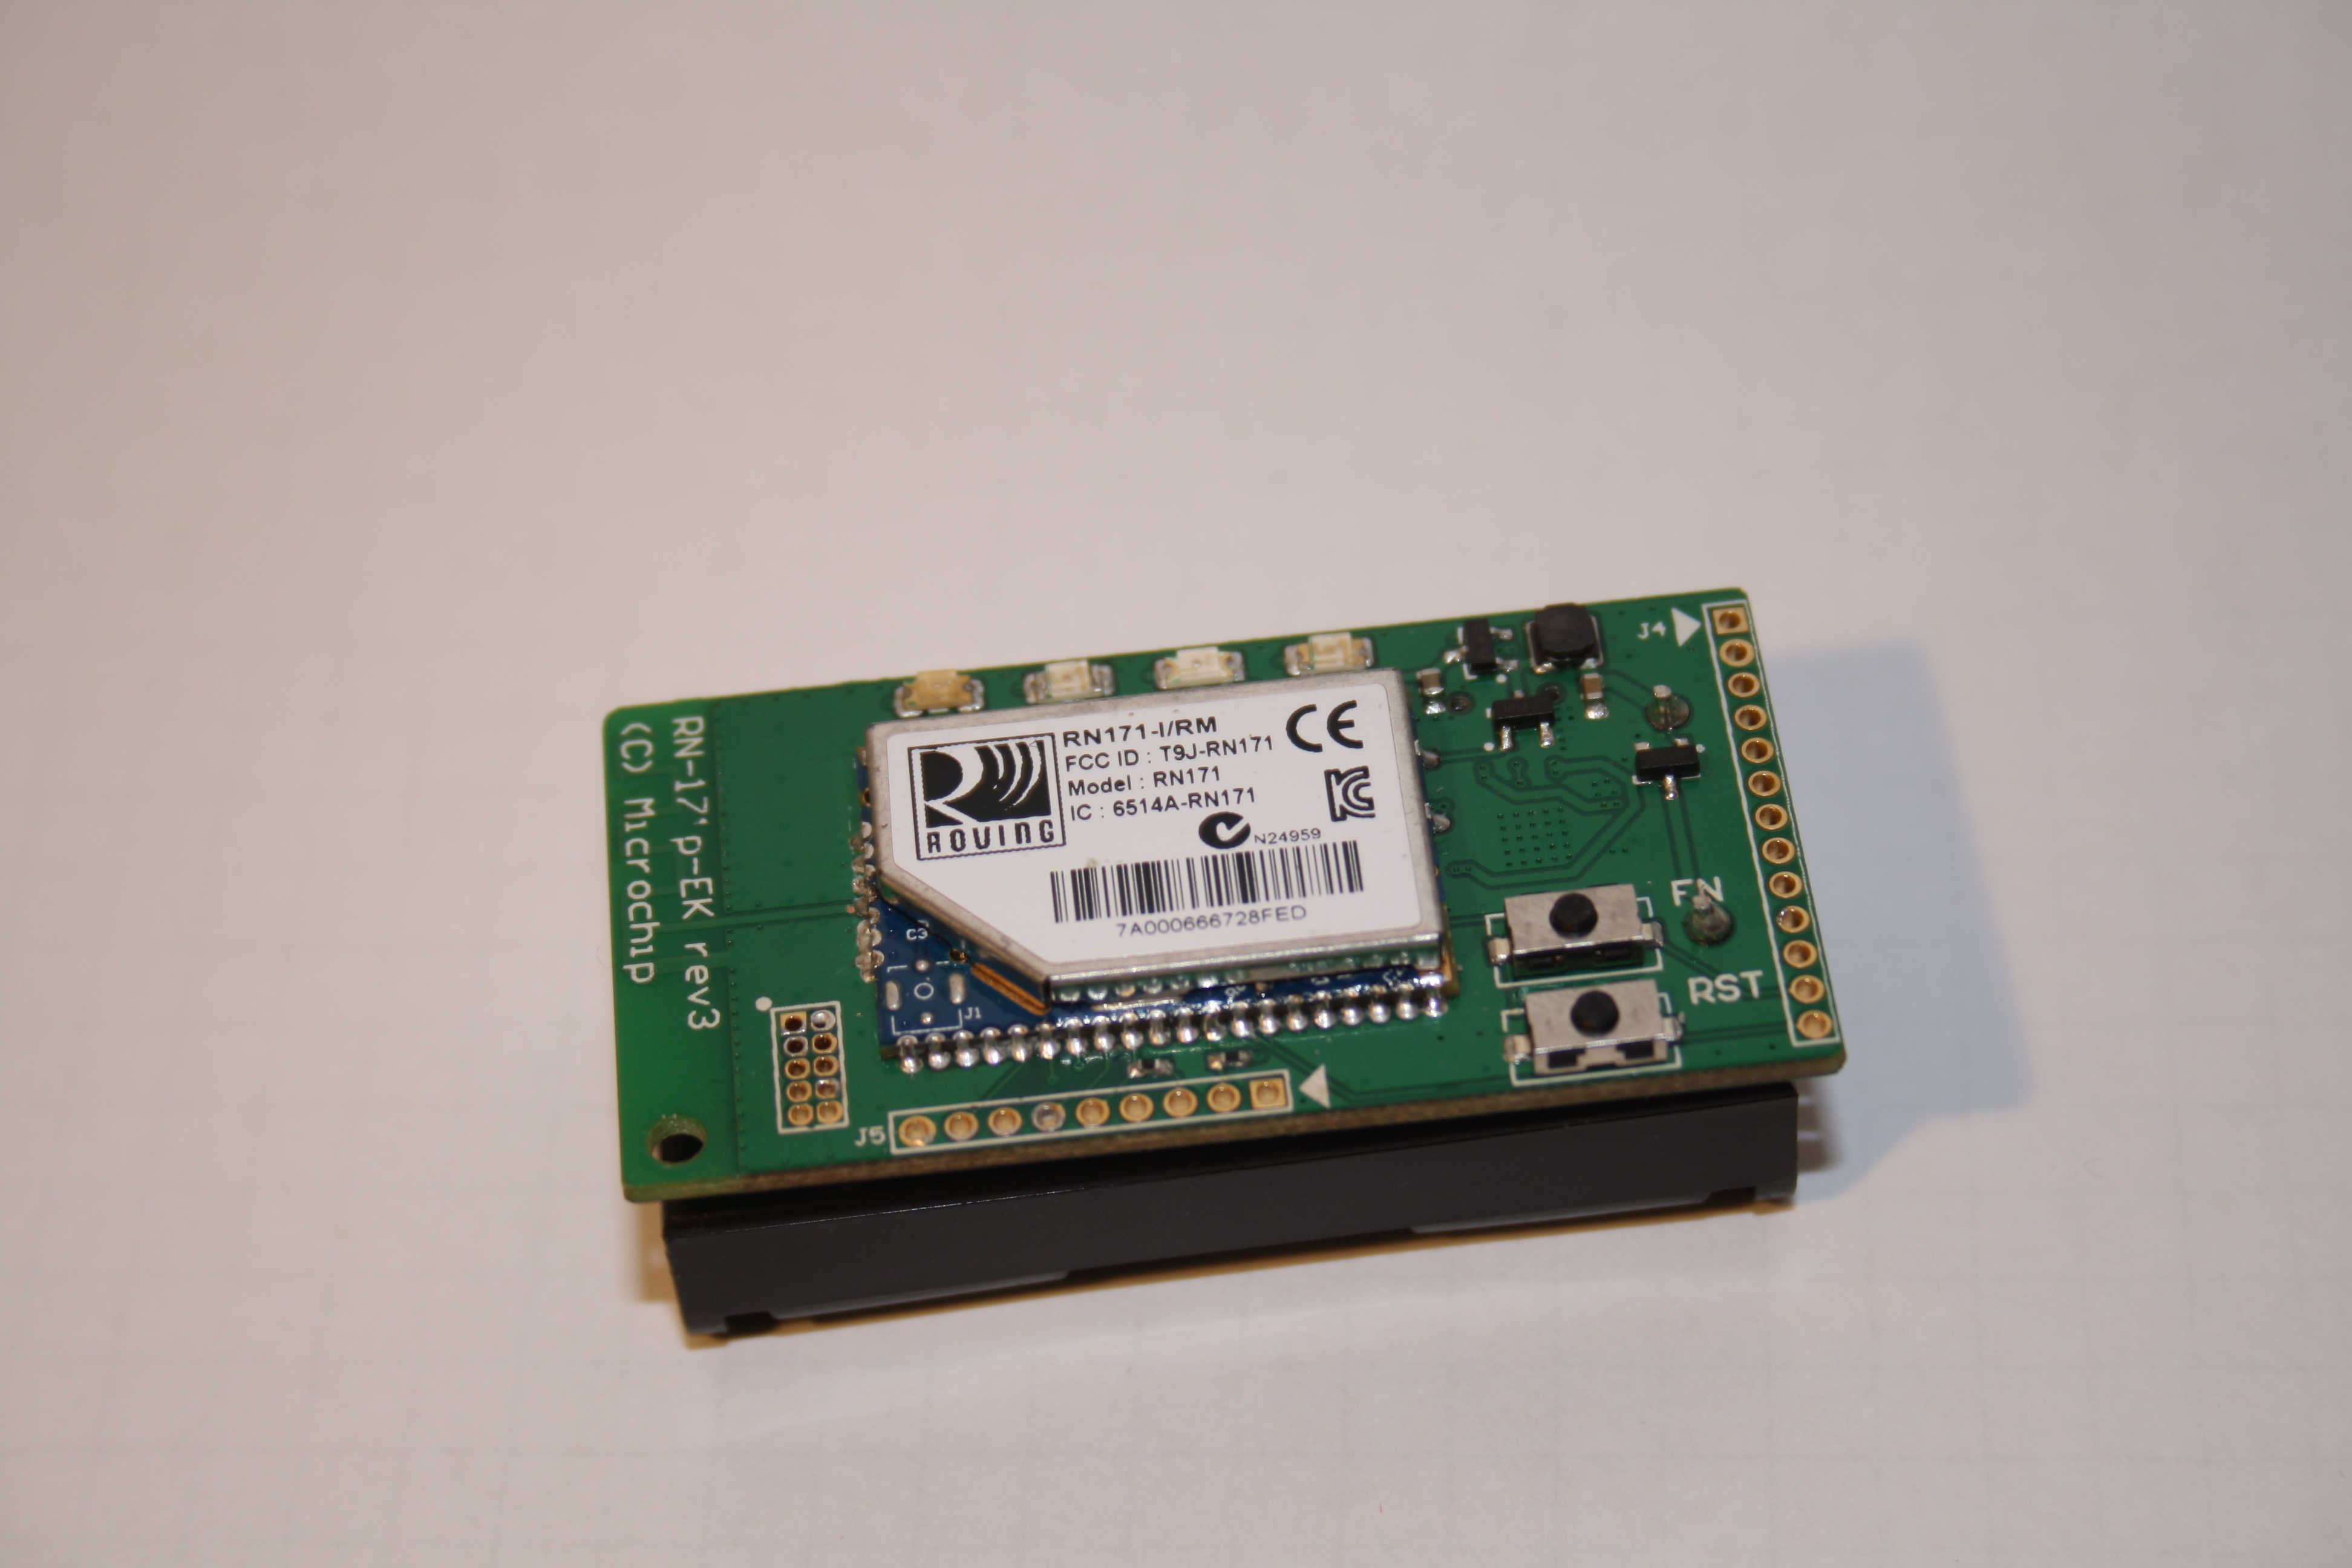
\includegraphics[width = 0.6\textwidth]{Bilder/RN171_EK}
    \par\end{centering}
    \caption[RN171 Evaluation-Kit]{RN171 Evaluation-Kit\cite{RN171_EK_source}}
    \label{RN171_EK}
  \end{figure}

  Um das WLAN-Modul so einzustellen, dass es sich Pin-gesteuert mit einem Host verbindet sind einige Schritte notwendig:
  \begin{itemize}
    \item \textbf{\$\$\$}\\
    Öffnet den Commandmode, nun können die Einstellungen vorgenommen werden
    \item \textbf{set wlan ssid <network\_name>}\\
    Deklariert den Netzwerknamen
    \item \textbf{set wlan phrase <network\_passphrase>}\\
    Deklariert das Passwort mit dem das Netzwerk gesichert ist
    \item \textbf{set ip host <host\_ip-address>}\\
    Deklariert die IP-Adresse des Empfängers
    \item \textbf{set ip remote <host\_portnumber>}\\
    Deklariert den Port auf dem der Empfänger die Daten empfangen soll
    \item \textbf{set sys iofunc 0x70}\\
    Durch diese Einstellung kann das WLAN-Modul über die Pins gesteuert werden
    \item \textbf{set wlan join 1}\\
    Stellt das WLAN-Modul auf automatisches Verbinden mit dem angegebenen Netzwerk ein
    \item \textbf{set ip protocol 4}\\
    Stellt das WLAN-Modul auf eine TCP/IP-Verbindung ein bei der nur Daten vom gespeicherten Host akzeptiert werden
    \item \textbf{set uart baud <desired-baudrate>}\\
    Stellt die Baudrate des WLAN-Moduls ein, Standard ist 9600
    \item \textbf{save}\\
    Speichert die Parameter in den Standardeinstellungen die nach einem Neustart geladen werden
    \item \textbf{reboot}\\
    Erzeugt einen Neustart bei dem die Standardeinstellungen geladen werden
  \end{itemize}
  Nachdem das WLAN-Modul auf die nötigen Parameter eingestellt ist, kann es direkt mit dem Mirkocontroller verbunden werden, die Verbidnung kann über einzelne Pins kontrolliert
  werden.

  \subsection{Herausforderungen und Lösungen}
  Eine Herausforderung stellte die Frage dar wie genau die Verbindung hergstellt wird. Das Datenblatt des WLAN-Moduls mit über 100 Seiten bietet viele potentielle Möglichkeiten.
  Die erste Wahl fiel auf das Auslesen einer Website, auf den ersten Anblick funktionierte das auch, jedoch musste festgestellt werden, dass unabhängig von der Website sehr ähnliche
  Daten verarbeitet werden, jedoch nicht der eigentliche Inhalt der Website sondern Providerinformationen.

  Die zweite Wahl fiel auf eine TCP/IP Verbindung, lediglich die genaue Umsetzung dieser ließ viele Möglichkeiten offen. Einerseits besteht die Möglichkeit eine Verbindung direkt
  über die Eingabe "open" im Commandmode zu öffnen, andererseits jedoch auch über die Pins als auch automatische Timeouts.

  Aufgrund der Einfachheit und vollen Kontrolle viel die Wahl auf die Ansteuerung über die Pins.
  Dazu stehen 3 unterschiedliche Pins zur Verfügung:
  \begin{itemize}
    \item \textbf{Associated}\\
    Mit einem Netzwerk verbunden
    \item \textbf{Open TCP connection}\\
    Die Verbidnung zum Host herstellen
    \item \textbf{Connected}\\
    Die Verbindung zum Host ist hergestellt
  \end{itemize}
  Die Statusinformationen Associated als auch Connected werden von dem WLAN-Modul geliefert, die Anweisung eine Verbindung herzustellen von dem Mirkocontroller.

%%%%%%%%%%%%%%%%%%%%%%%%%%%%%%%%%%%%%%%%%%%%%%%%%%%%%%%%%%%%%%%%%%%%%%%%%%%%%%%
\section{Schnittstelle Applikation}


  \subsection{Technische Planung}
  
      \subsubsection{Eclipse}
    
Eclipse, entwickelt von der Eclipse Foundation, ist ein Open Source Programmierwerkzeug. Ursprünglich wurde es als integrierte Entwicklungsumgebung für die Programmiersprache Java entwickelt, heutzutage wird es jedoch auch zur Bewältigung einiger anderer Entwicklungsaufgaben verwendet.

    \subsubsection{JDBC}
    
The Java Database Connectivity (JDBC) API is the industry standard for database-independent connectivity between the Java programming language and a wide range of databases  SQL databases and other tabular data sources, such as spreadsheets or flat files. The JDBC API provides a call-level API for SQL-based database access.
JDBC technology allows you to use the Java programming language to exploit "Write Once, Run Anywhere" capabilities for applications that require access to enterprise data. With a JDBC technology-enabled driver, you can connect all corporate data even in a heterogeneous environment.


  \subsection{Umsetzung}

  \subsection{Herausforderungen und Lösungen}
